\section{Trends in Identity Theft from 2008-2021}
\label{app:longitudinal}

Beyond the average characteristics over the entire study period of 2008 to 2021, examining the trends year by year reveals shifts in the type of theft, as well as how victims experience them. Figures  \ref{fig:theft_type_long} and \ref{fig:discovery_method_long}  illustrate these patterns, showing how the crime itself, the way victims discover it, and its financial impact have changed from 2008 to 2021. 

First, considering the types of identity theft experienced, Figure \ref{fig:theft_type_long} shows a shift from traditional financial account misuse to other forms, which is particularly evident in the most recent survey year, 2021. As shown, existing bank account or credit card misuse remain the most common types of identity theft experienced. Misuse of existing credit cards, historically the most prevalent type (affecting over 50\% of victims in some years), saw a substantial decline between 2018 and 2021, dropping to roughly 38\%. Existing bank account misuse followed a similar pattern, also decreasing significantly in 2021. In contrast, the category of "Other Existing Account Misuse," which includes misuse of online accounts like email or social media, experienced a dramatic surge in 2021, rising from around 10\% in 2018 to over 30\% of victims in 2021. This indicates a significant change in criminal activity towards compromising online credentials. This could also be due to the rapid rise of social media over the last few years. New account fraud and other misuses of personal information remained relatively stable at lower prevalence levels throughout the period.


\begin{figure}[htbp]
    \centering
    % --- Subfigure A: Counts ---
    \begin{subfigure}[b]{0.48\textwidth}
        \centering
        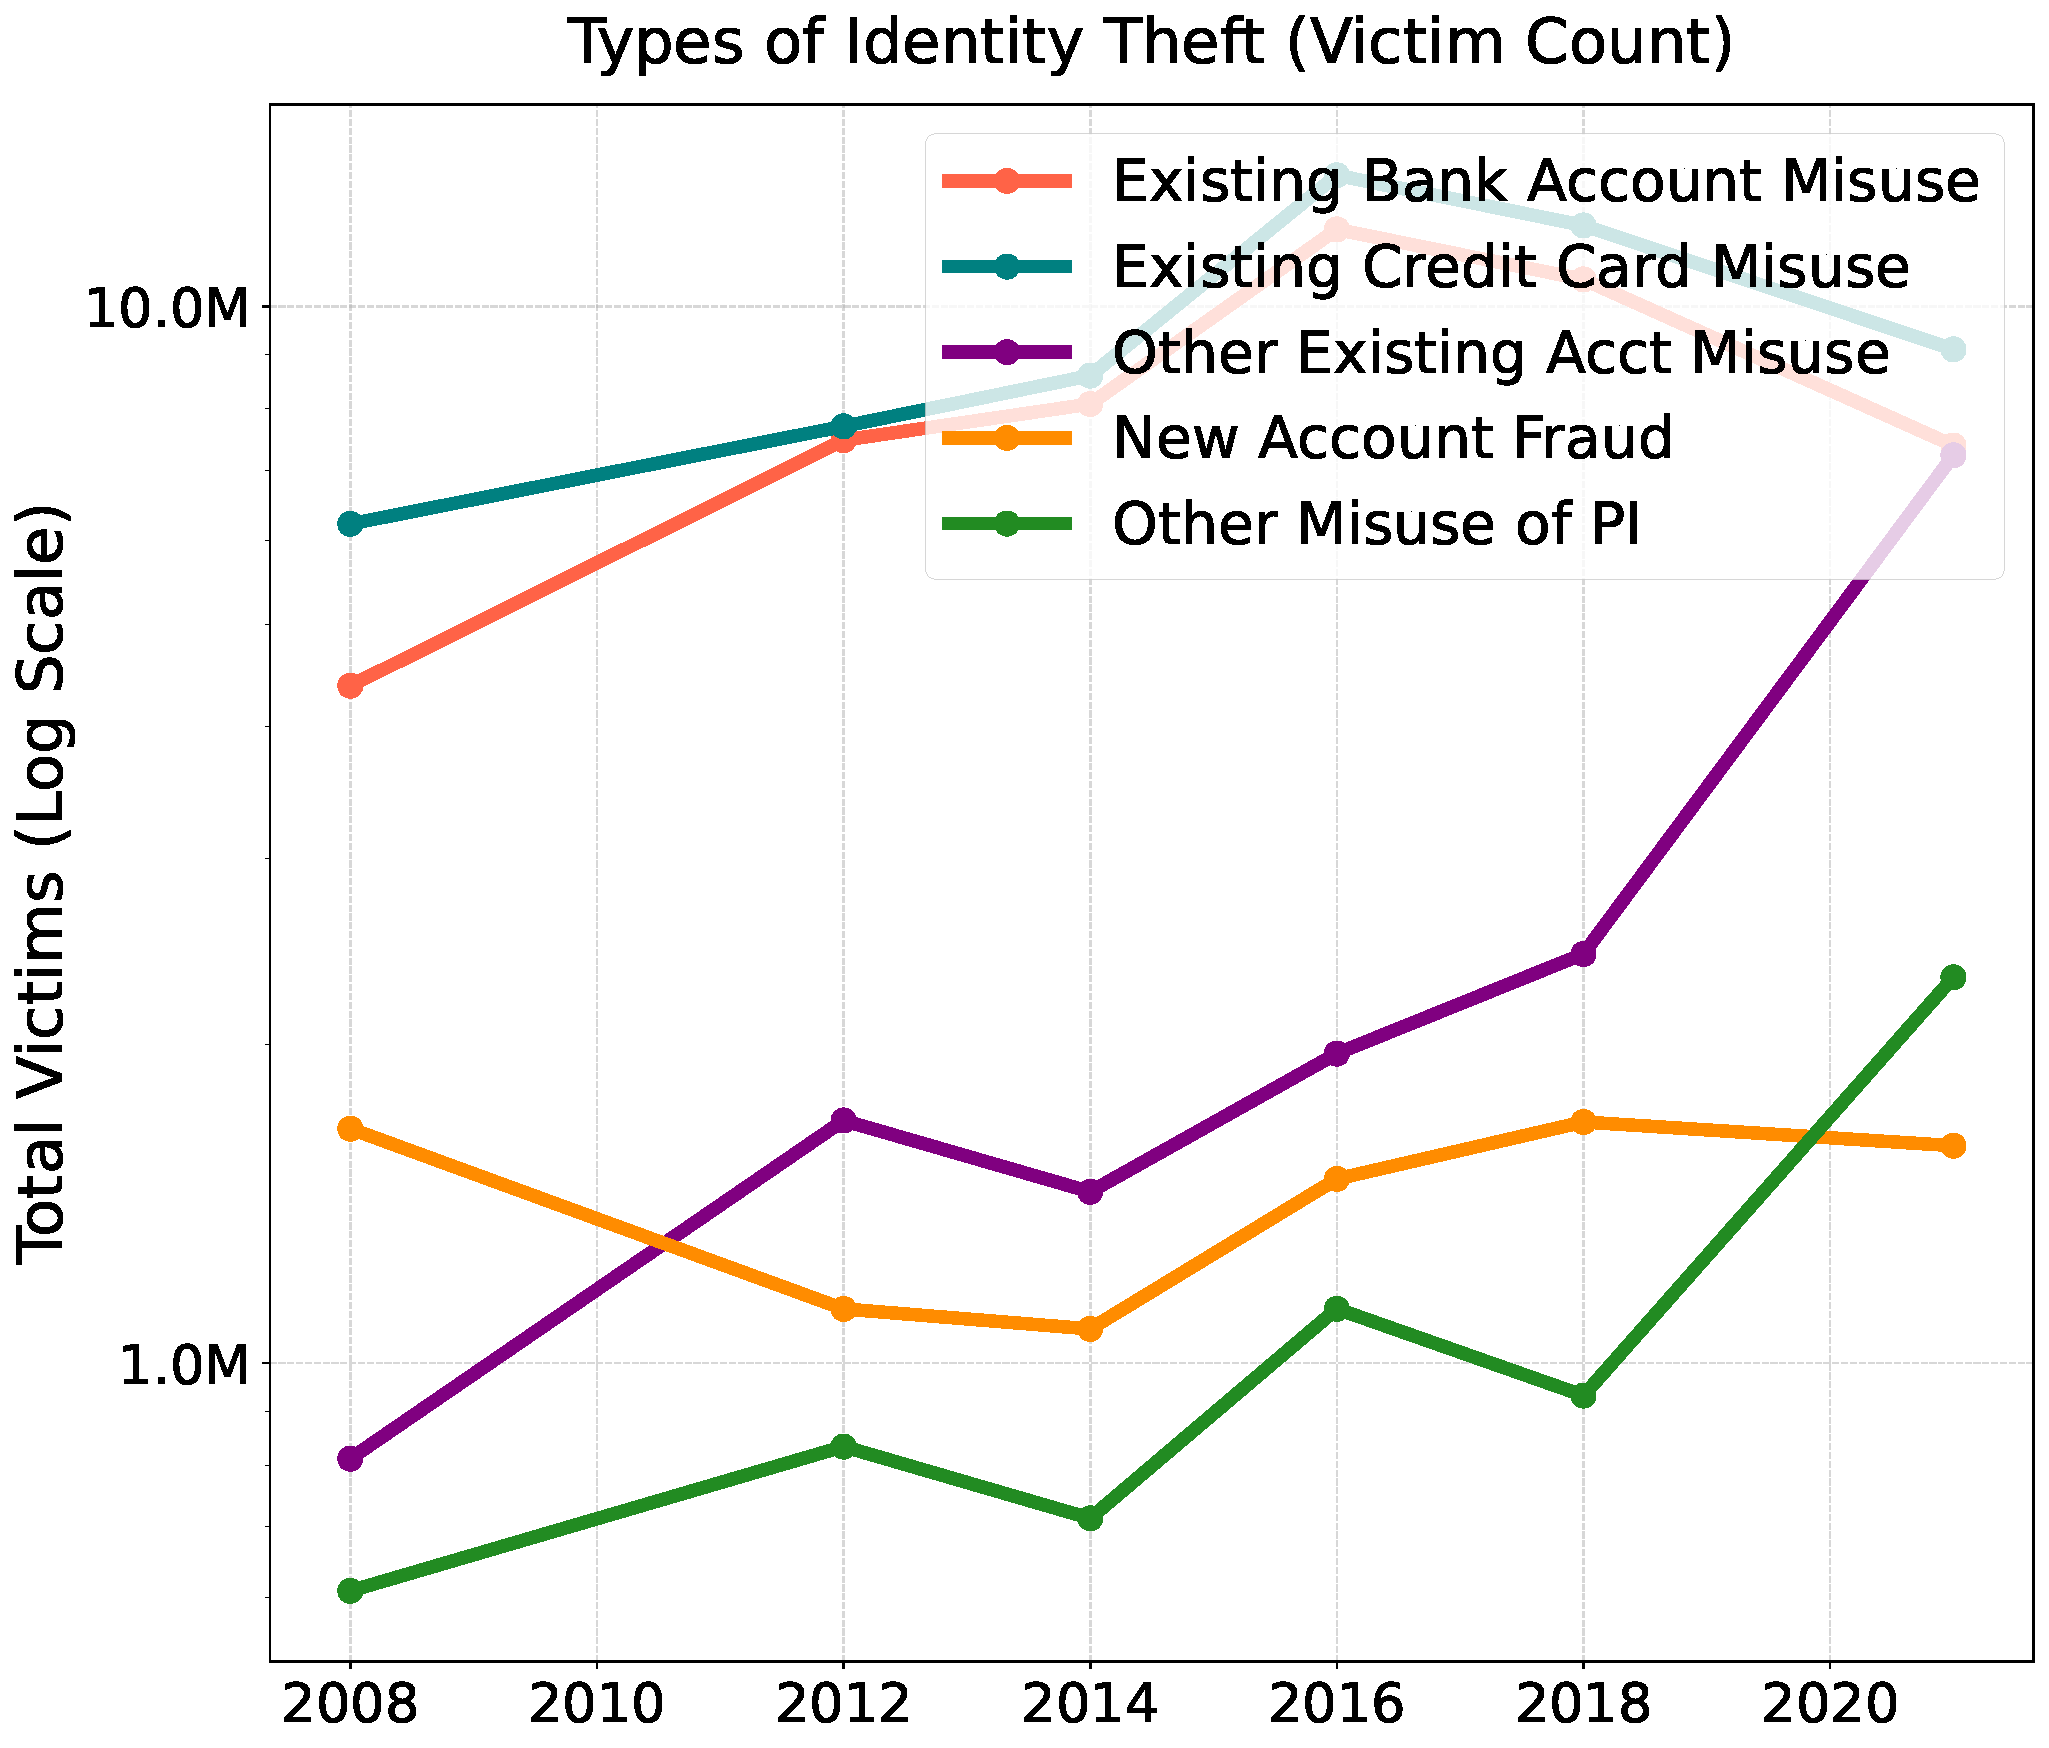
\includegraphics[width=\textwidth]{figures/incident_trends/plot2_theft_types_count.pdf}
        \caption{Number of victims categorized by the type of identity theft they suffered from.}
        \label{fig:theft_type_long_a}
    \end{subfigure}
    \hfill
    % --- Subfigure B: Percentages ---
    \begin{subfigure}[b]{0.48\textwidth}
        \centering
        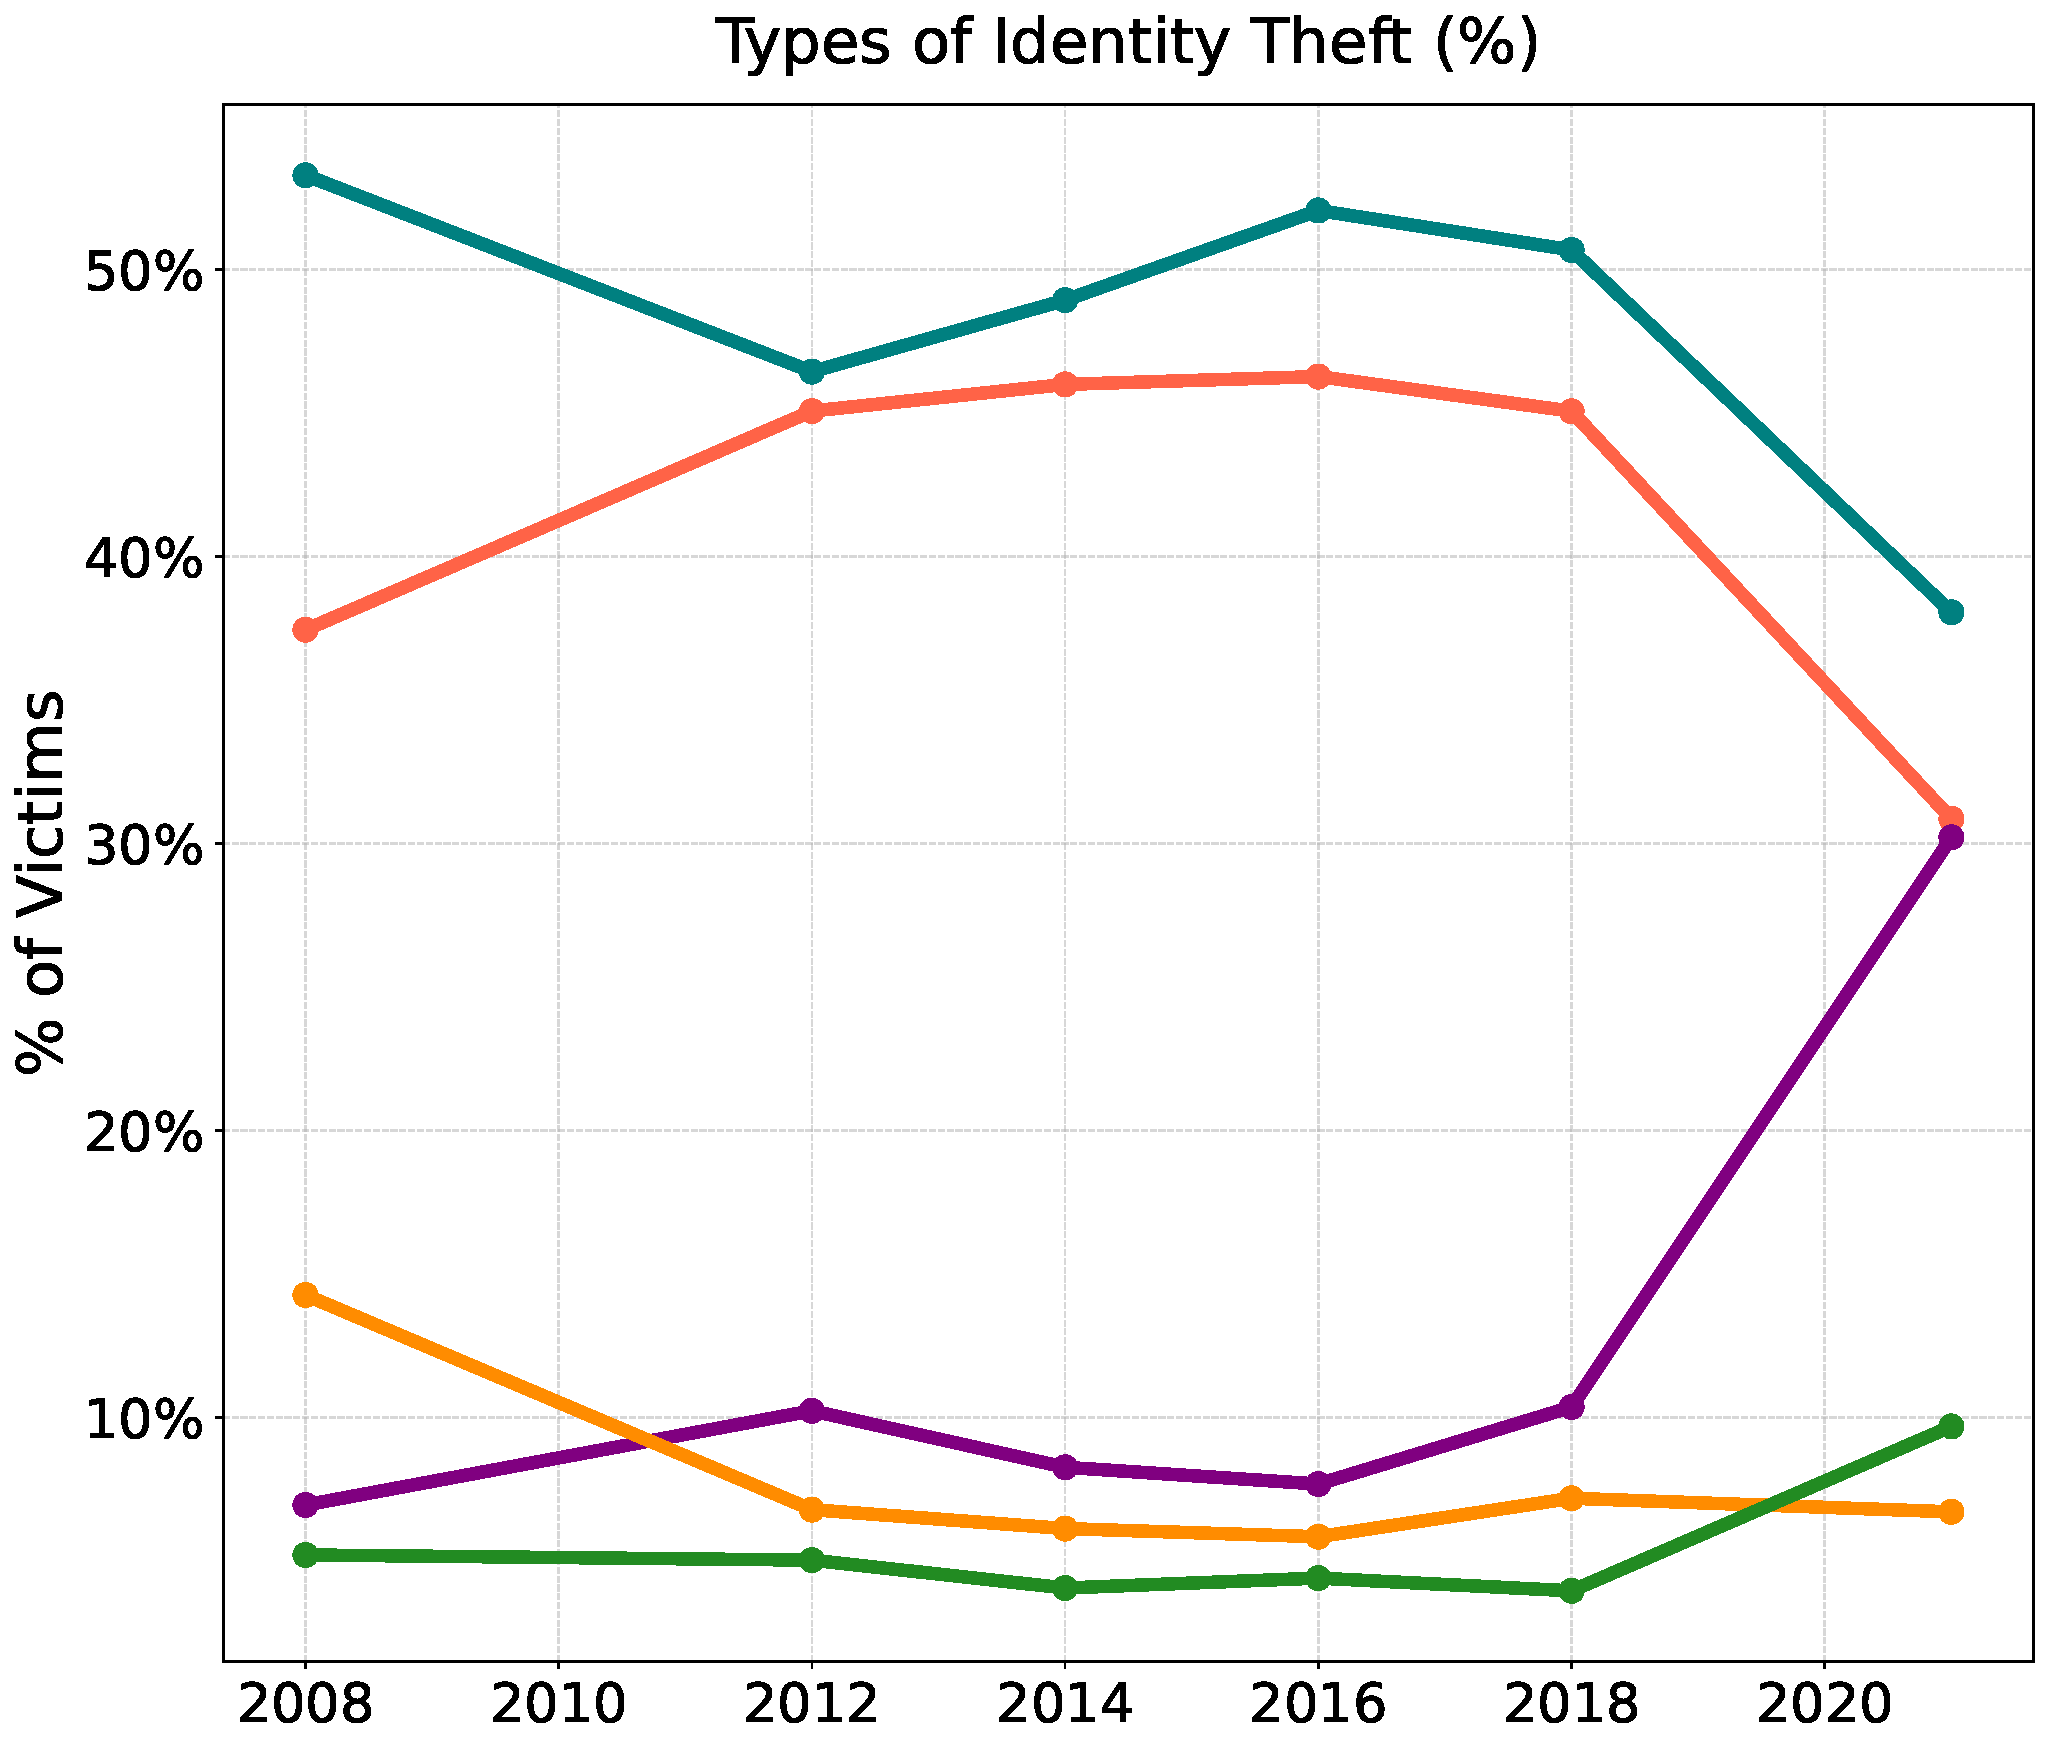
\includegraphics[width=\textwidth]{figures/incident_trends/plot2_theft_types_percentage.pdf}
        \caption{Percentage of victims categorized by the type of identity theft they suffered from.}
        \label{fig:theft_type_long_b}
    \end{subfigure}
    
    \caption{Analysis of theft types over the longitudinal study period.}
    \label{fig:theft_type_long}
\end{figure}

% Figure \ref{fig:theft_method_long} displays how victims reported their information was obtained by offenders, which adds more context to the nature of the crime they suffered. A noticeable trend is the considerable decline in information being compromised during a transaction. This method, although always the most common identified theft method, peaked in 2012 and 2014, and then fell sharply after, accounting for less than 8\% in 2021. Note that in October 2015, the major credit card networks (Europay, MasterCard, and Visa) implemented the EMV liability shift, a policy change that transferred financial responsibility for in-person counterfeit card fraud from the card issuer to whichever party in the transaction (either the merchant or the issuer) had not adopted the more secure chip card technology. This was not a government mandated law but rather a policy change by the major credit card networks to financially incentivize the adoption of chip technology. The policy forced a nationwide payment infrastructure upgrade in an effort to counter the vulnerability of the easily cloned magnetic strip, which had been a leading carrier of counterfeit card fraud. The EMV liability shift was a major turning point in the fight against in-person payment fraud. The reduction in information being stolen during a transaction in Figure \ref{fig:theft_method_long} aligns with the time frame of the October 2015 liability shift for EMV chip card adoption in the United States. The efficacy of this transition was reported by the Federal Reserve, which reported that in-person card fraud, including counterfeit cards, declined from \$3.68 billion in 2015 to \$2.91 billion in 2016 \cite{fed2018fraud}. Similarly, Visa also reported that by October 2016, counterfeit fraud dollars at chip enabled merchants had dropped by 43\% compared to a year earlier \cite{visa2016infographic}, and later data showed this decline reached 66\% by June 2017 \cite{visa2017report}.

% \begin{wrapfigure}{r}{0.5\textwidth}
%     \centering
%     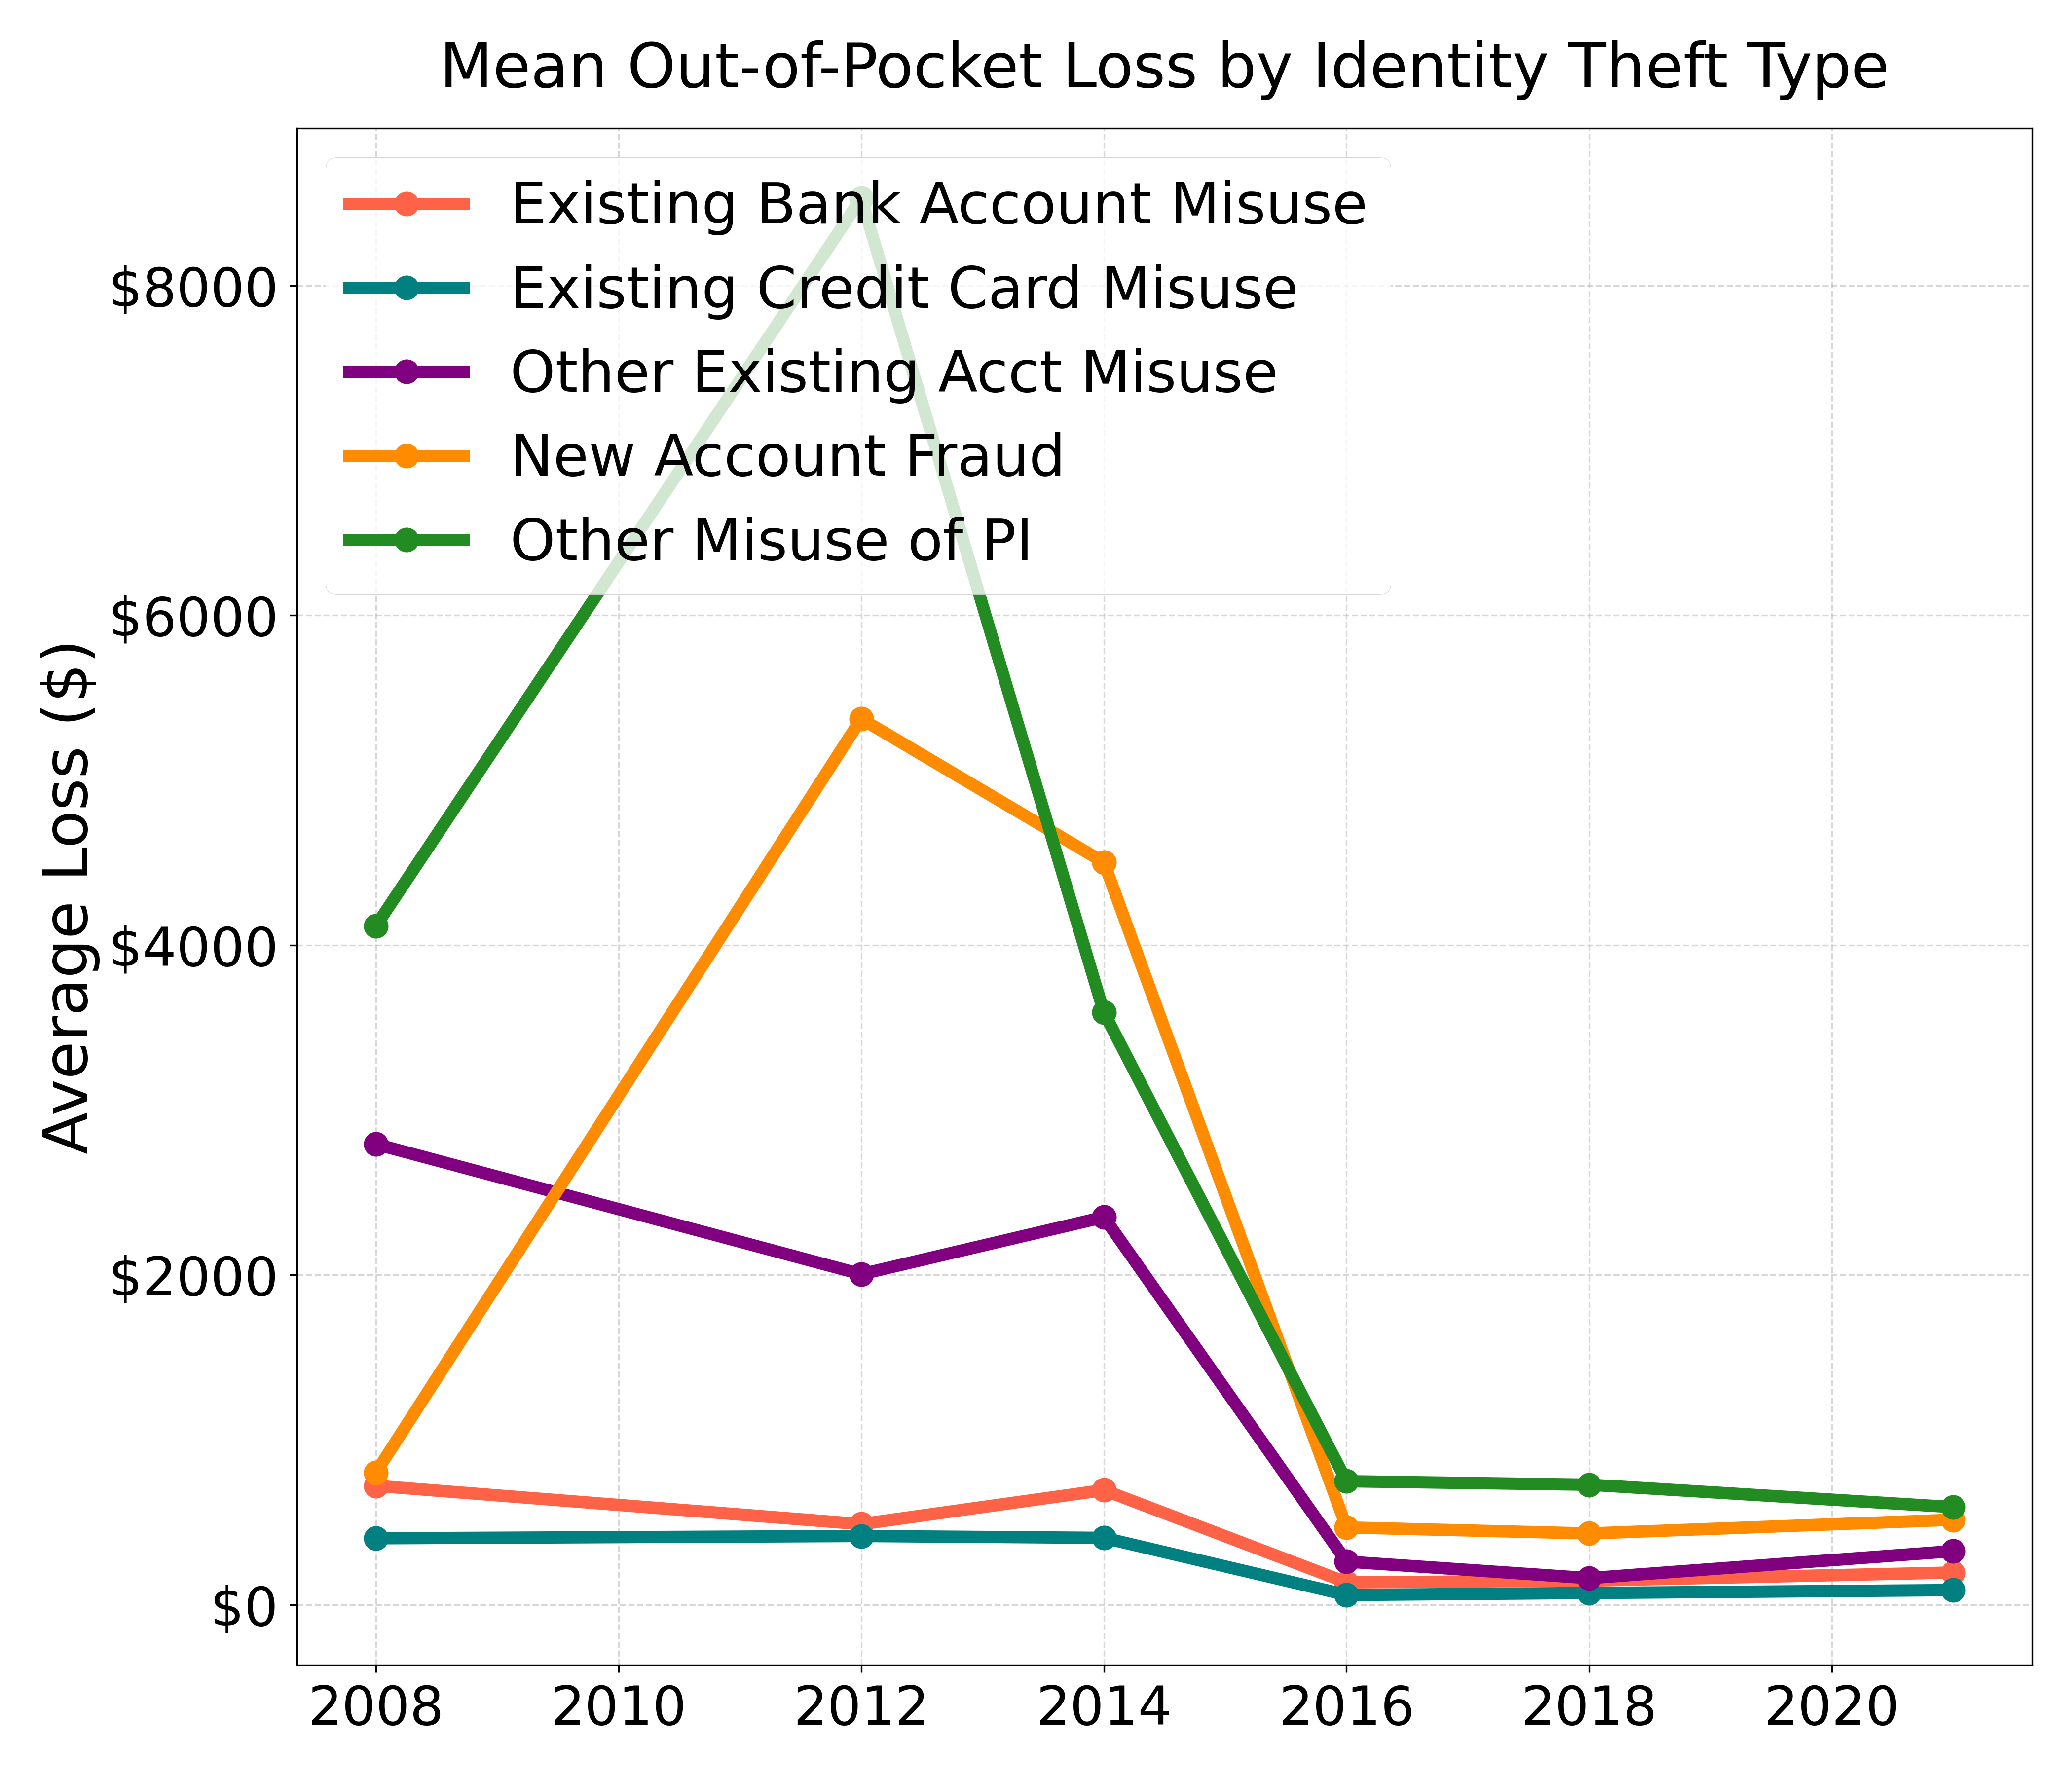
\includegraphics[width=0.48\textwidth]{figures/incident_trends/plot5_oop_loss_by_type.png}
%     \caption{Mean Out-of-Pocket Loss by Identity Theft Type (2008–2021).}
%     \label{fig:oop_loss_comparison}
% \end{wrapfigure}

Next, Figure \ref{fig:discovery_method_long} illustrates how victims became aware of the misuse, and its trends mirror the shift in crime types. "Notified by Bank," which rose significantly between 2008 and 2016 to become the most common discovery method (peaking at nearly 50\%), saw a sharp reversal, dropping considerably by 2021 to around 26\%. On the other hand, "Notified by Other Person/Organization," which began as a less common method, rose dramatically in 2021, increasing from roughly 6\% in 2018 to over 21\%. This aligns with the rise of social media and email account misuse as seen in Figure \ref{fig:theft_type_long}, suggesting victims are increasingly learning about compromises through their social networks or other non-financial organizations.


% \begin{figure}[htbp]
%     \centering
%     % --- Subfigure A: Counts ---
%     \begin{subfigure}[b]{0.48\textwidth}
%         \centering
%         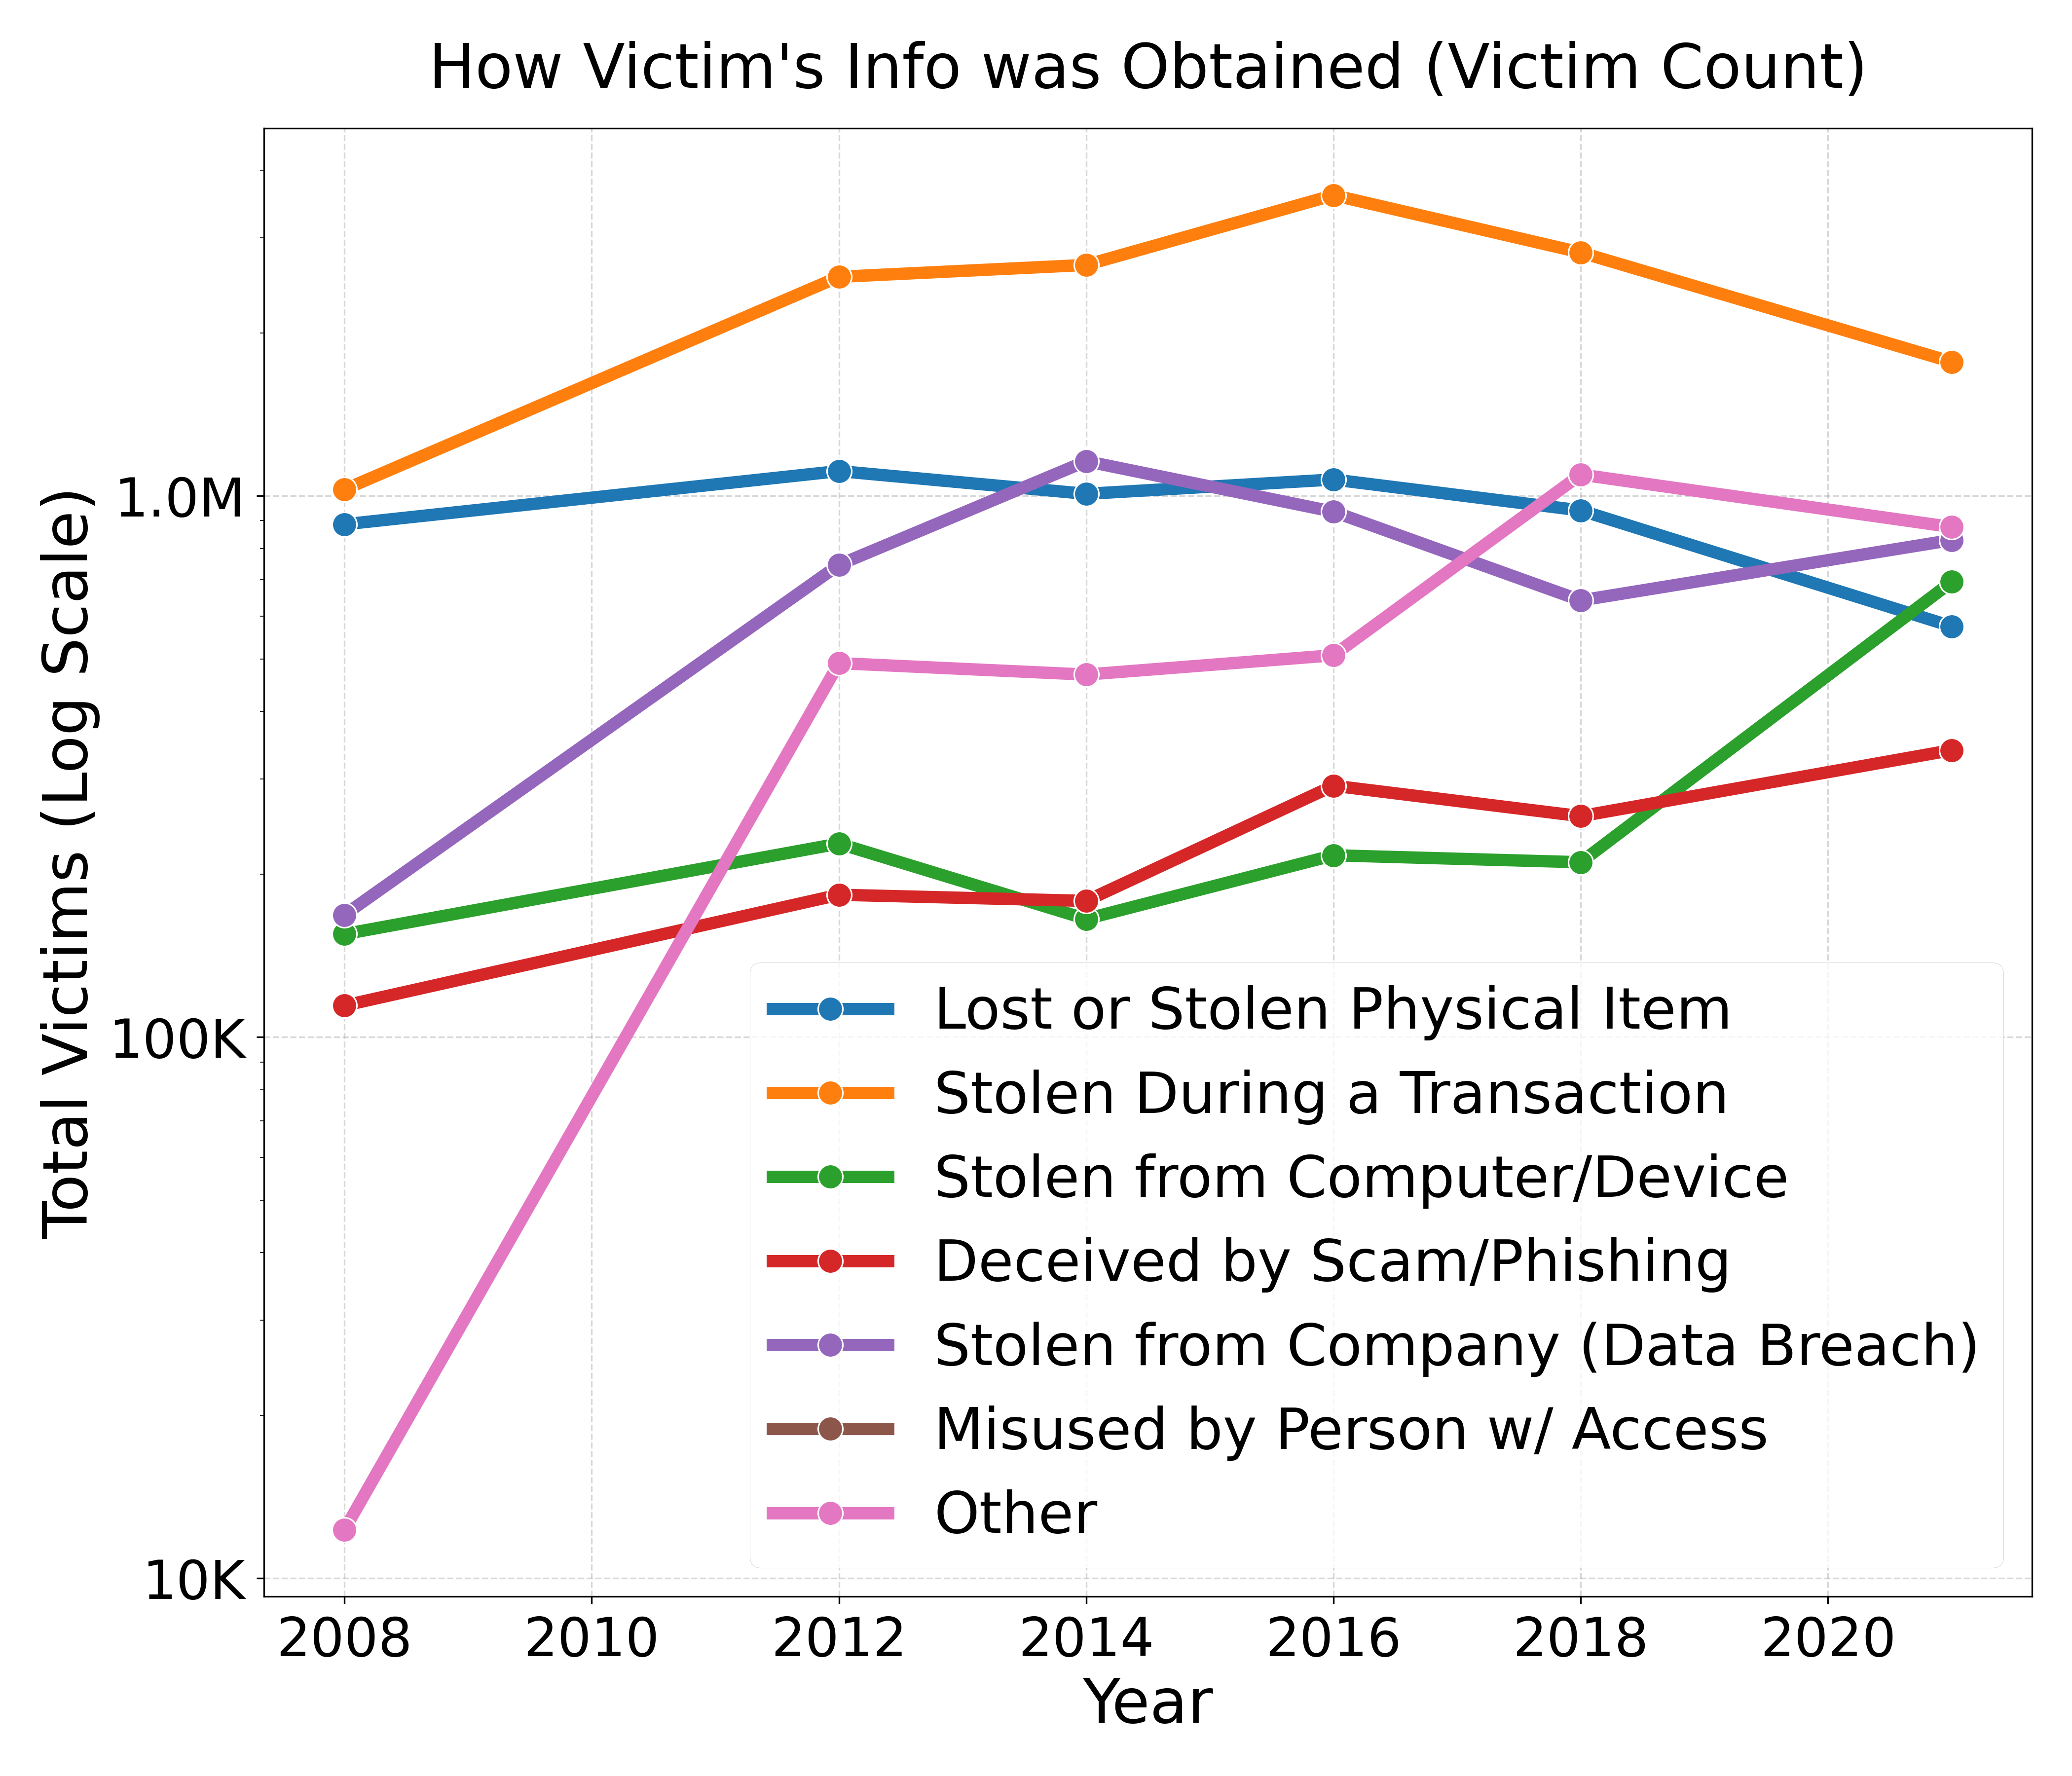
\includegraphics[width=\textwidth]{figures/incident_trends/plot1_theft_methods_count.png}
%         \caption{Number of victims categorized by how their information was stolen.}
%         \label{fig:theft_method_long_a}
%     \end{subfigure}
%     \hfill % Adds horizontal space between the two images
%     % --- Subfigure B: Percentages ---
%     \begin{subfigure}[b]{0.48\textwidth}
%         \centering
%         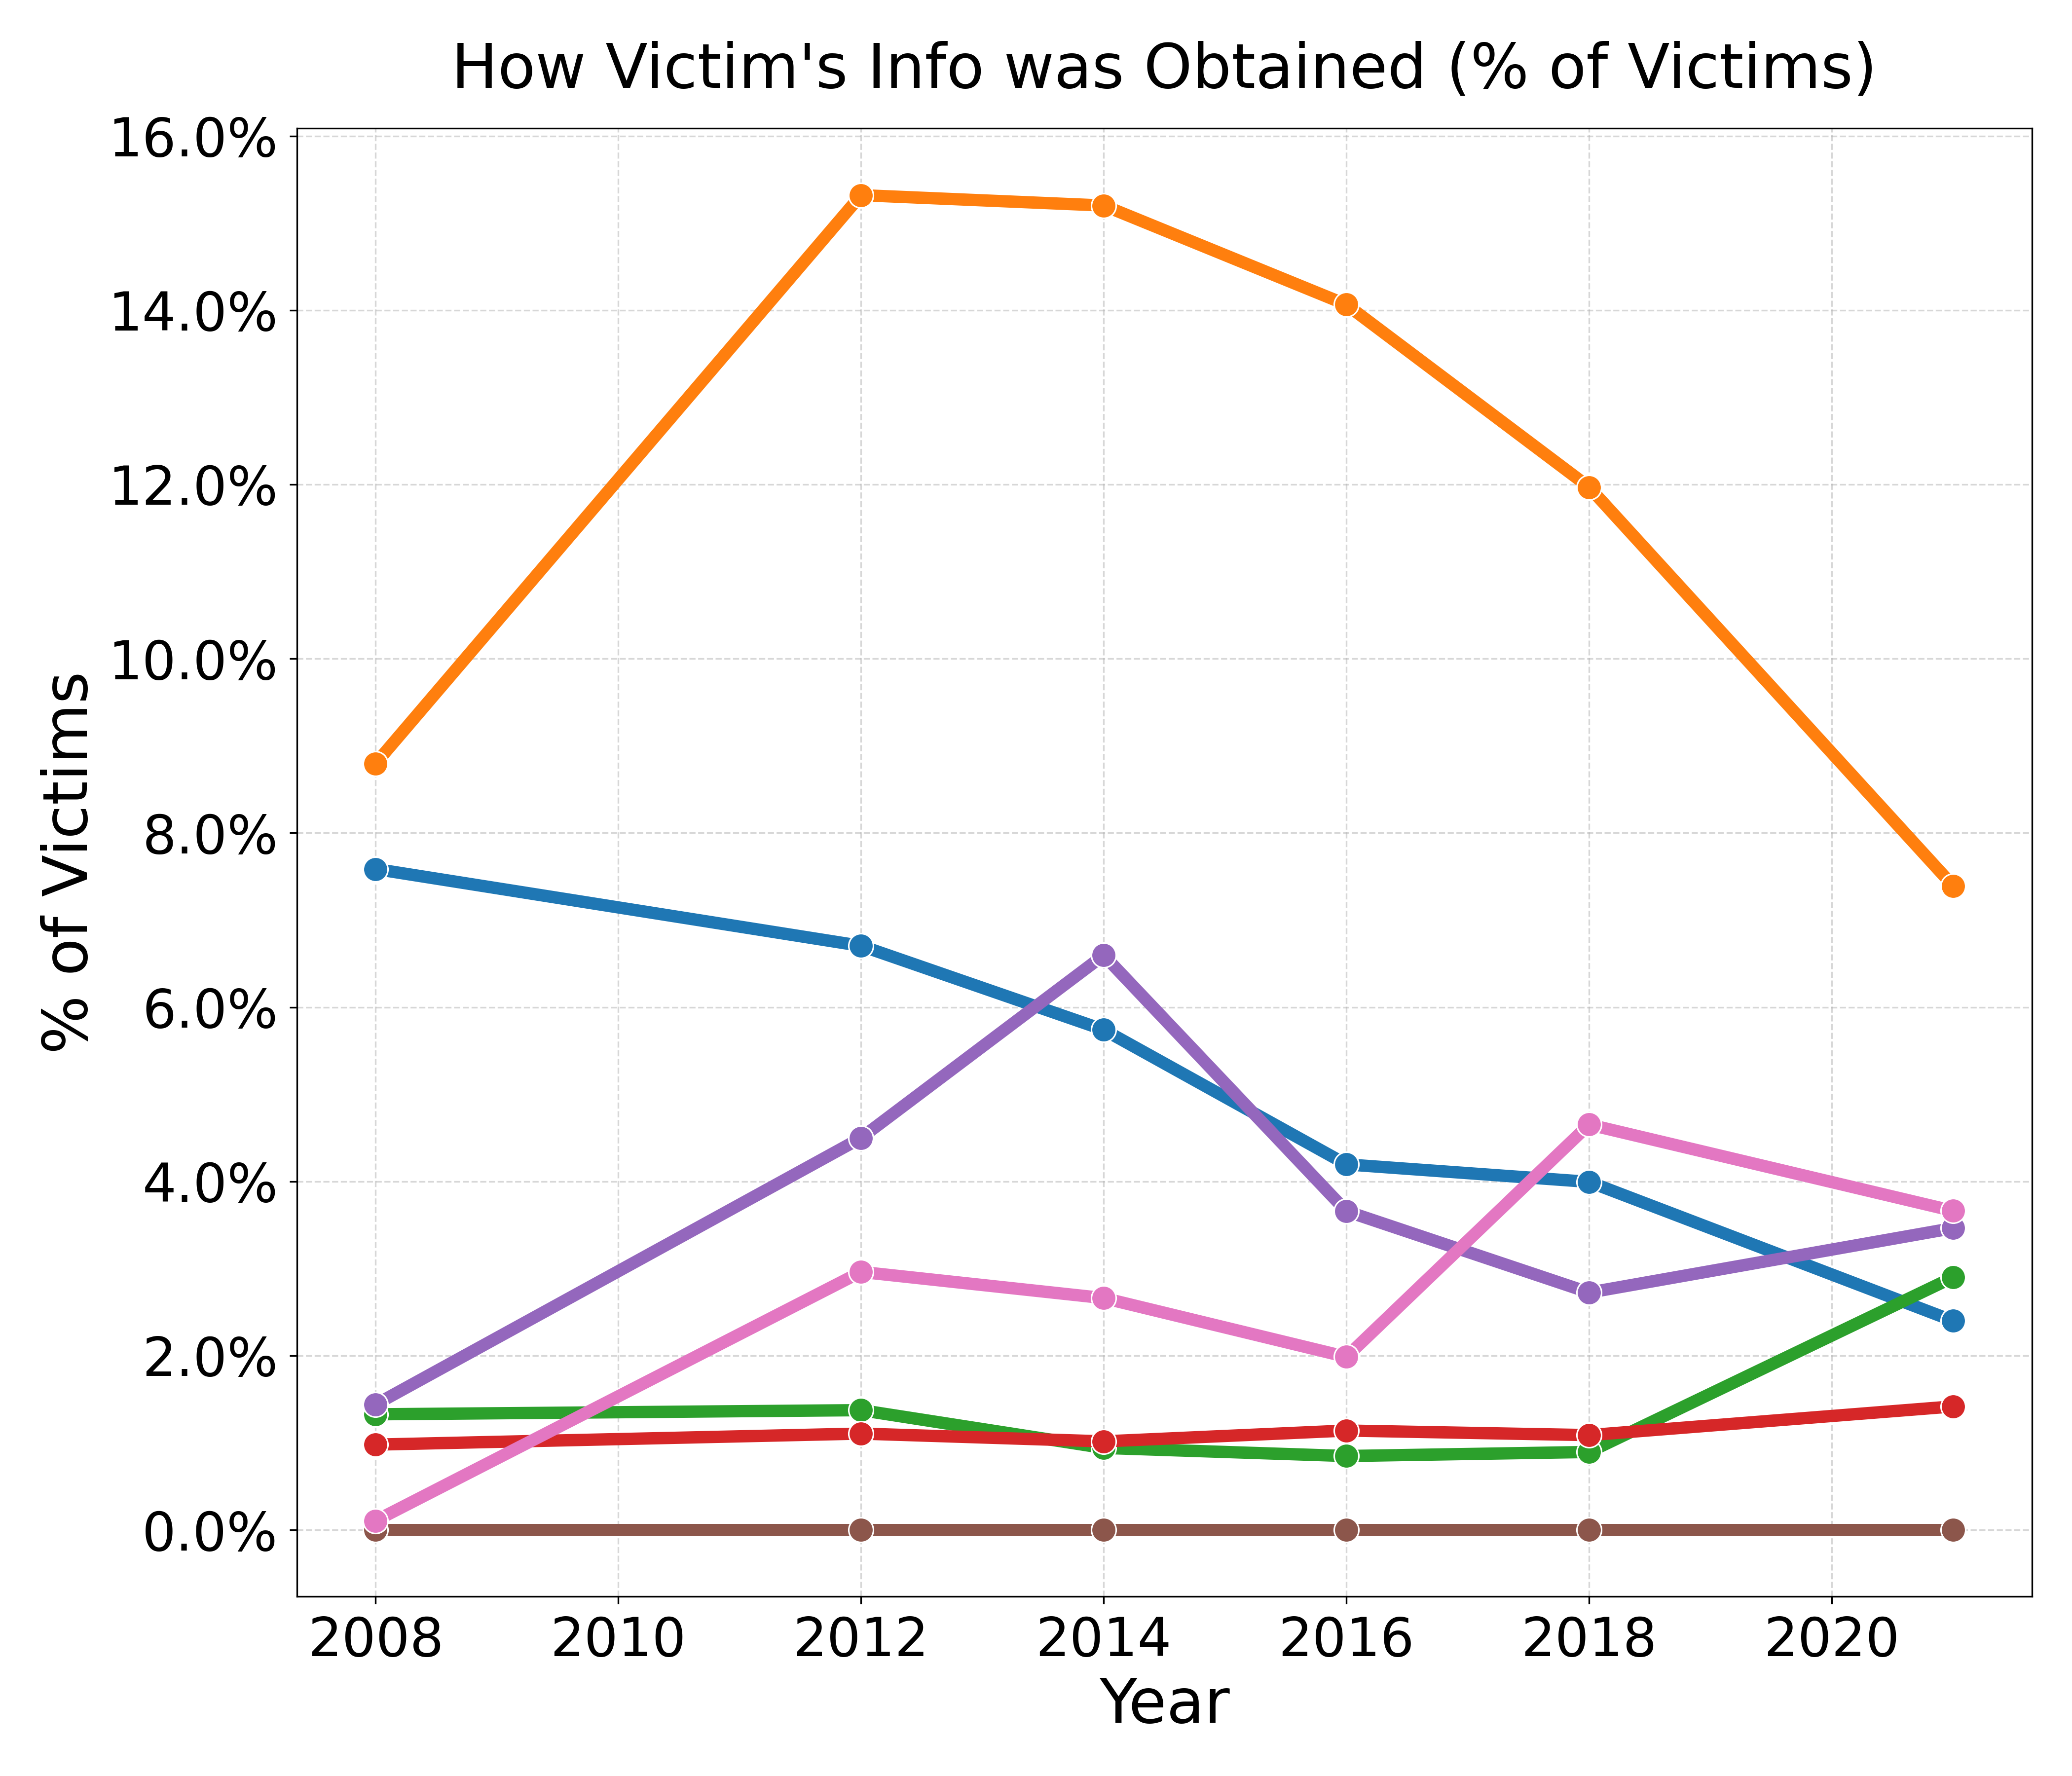
\includegraphics[width=\textwidth]{figures/incident_trends/plot1_theft_methods_percentage.png}
%         \caption{Percentage of victims categorized by how their information was stolen.}
%         \label{fig:theft_method_long_b}
%     \end{subfigure}
    
%     \caption{Analysis of theft methods over the longitudinal study period.}
%     \label{fig:theft_method_long}
% \end{figure}

\begin{figure}[htbp]
    \centering
    % --- Subfigure A: Counts ---
    \begin{subfigure}[b]{0.48\textwidth}
        \centering
        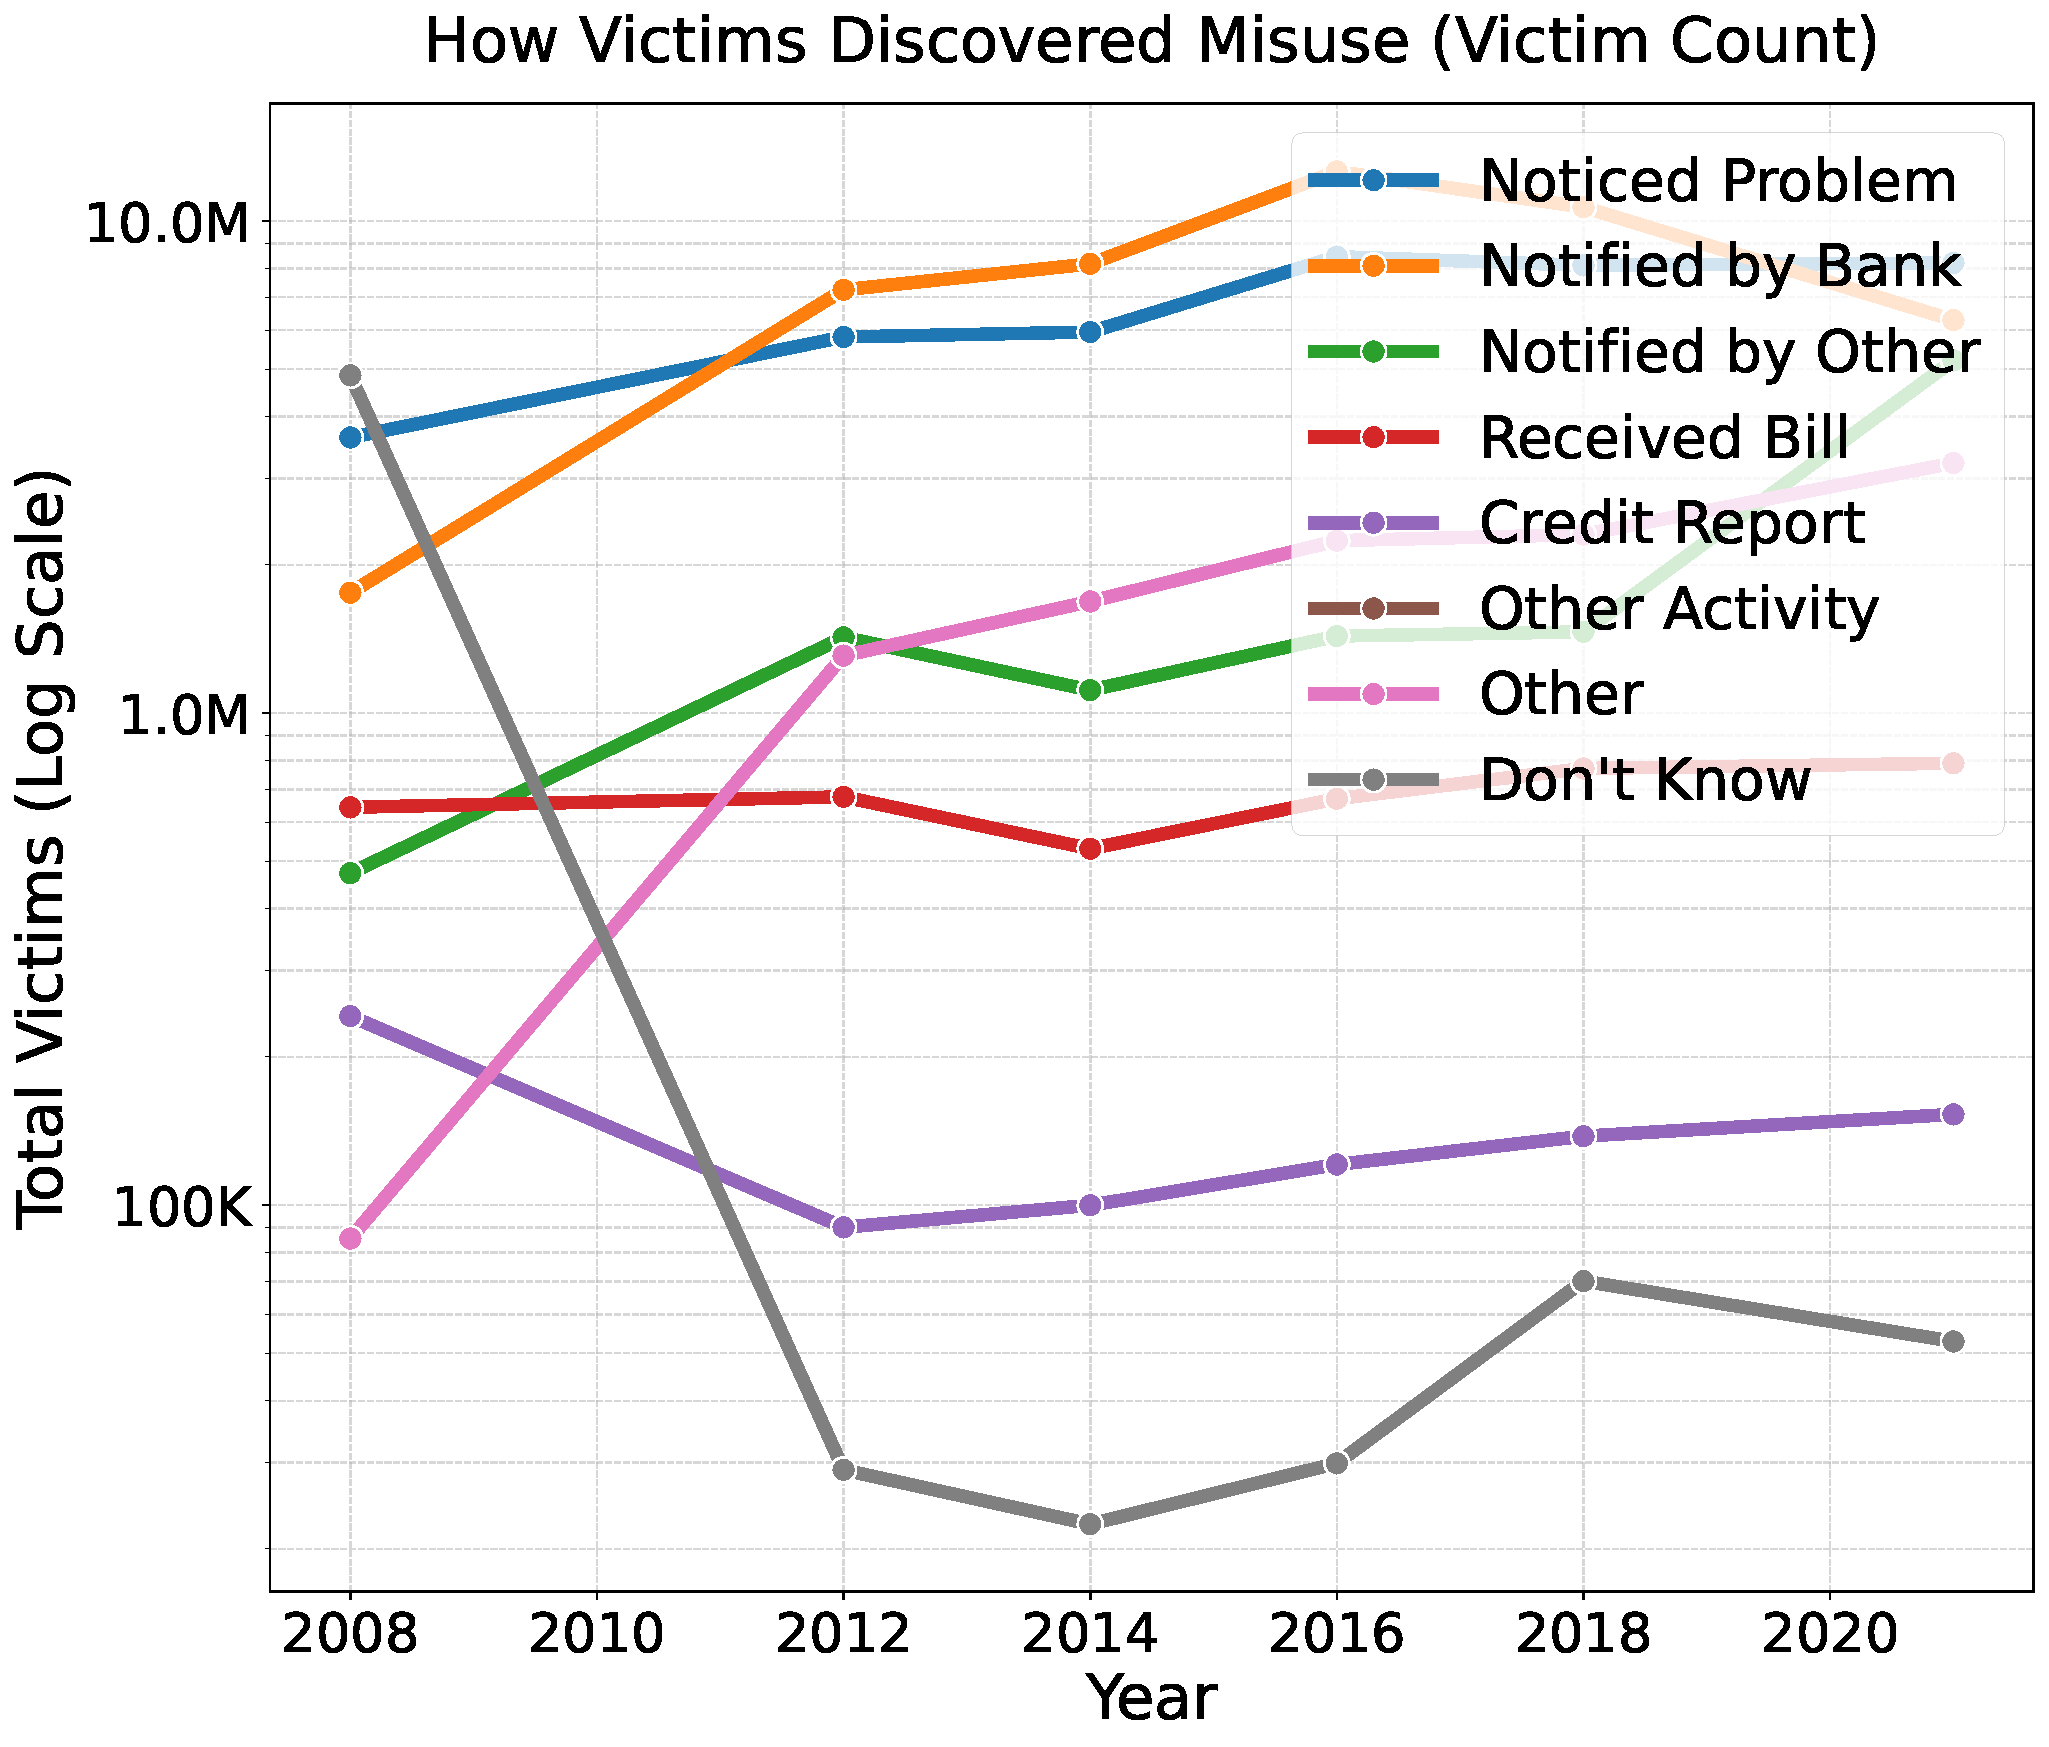
\includegraphics[width=\textwidth]{figures/incident_trends/plot3_discovery_count.pdf}
        \caption{Number of victims categorized by their discovery method.}
        \label{fig:discovery_method_long_a}
    \end{subfigure}
    \hfill
    % --- Subfigure B: Percentages ---
    \begin{subfigure}[b]{0.48\textwidth}
        \centering
        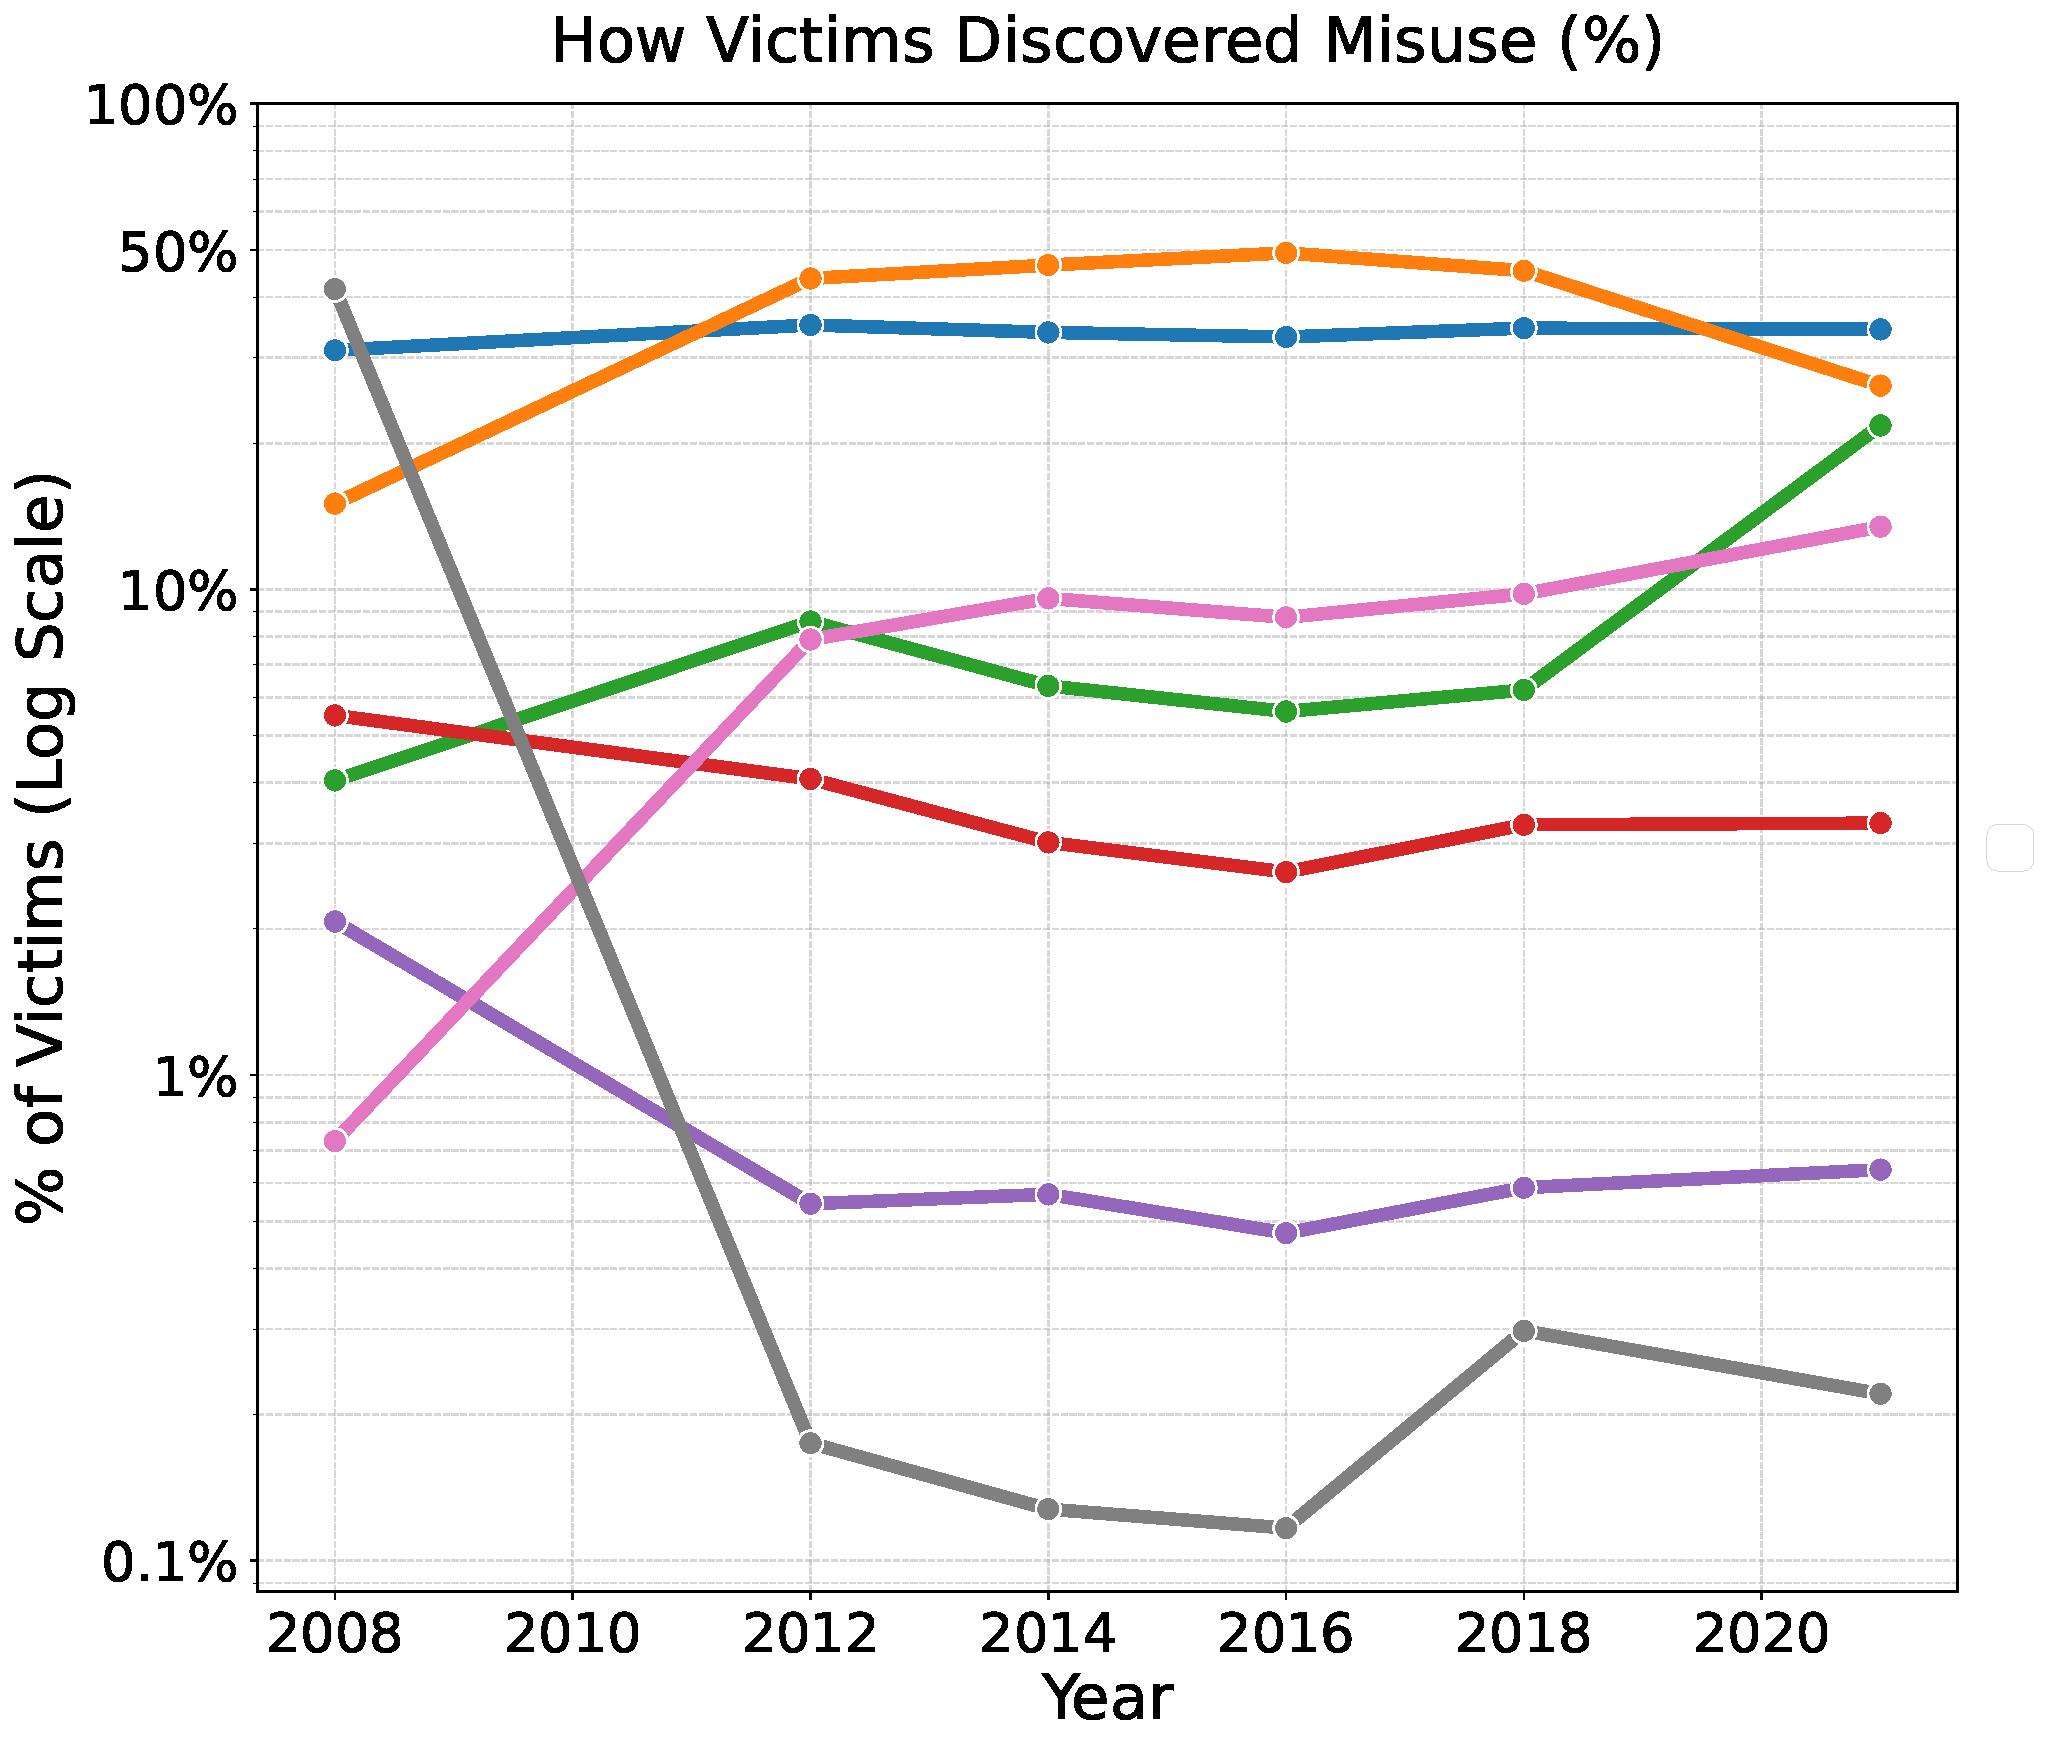
\includegraphics[width=\textwidth]{figures/incident_trends/plot3_discovery_percentage.pdf}
        \caption{Percentage of victims categorized by their discovery method.}
        \label{fig:discovery_method_long_b}
    \end{subfigure}
    
    \caption{Longitudinal trends in how victims discovered the theft incidents.}
    \label{fig:discovery_method_long}
\end{figure}


% Finally, a financial trend is evident in Figure \ref{fig:oop_loss_comparison}, which compares the average out of pocket (OOP) losses adjusted to 2021 dollars, specifically for victims of existing credit card misuse versus existing bank account misuse. It is worth noting that our OOP loss is less than direct loss values noted by BJS official reports \cite{HarrellThompson2024}, because we include only costs that were not recoverable to the victim, rather than including reimbursed costs. Both categories show a dramatic drop in average OOP loss between 2014 and 2016. Figure \ref{fig:oop_loss_comparison} displays that all categories show a dramatic drop and convergence between 2014 and 2016. We present two hypothesized explanations for this trend. 



% First, for the existing bank account misuse and existing credit card misuse OOP loss, the EMV transition could have played a role, because it reduced the most common type of high value, card present fraud, and for the fraud that did occur, liability was clearer and banks had implemented faster detection systems, leading to more \$0 liability outcomes for consumers \cite{aba2018report}. Victims still reported "credit card misuse" because criminals pivoted to online, card not present fraud \cite{fed2018fraud}. This remote fraud is often more easily and quickly reimbursed by banks. Unlike in-person counterfeit fraud, where a dispute could be complex, in a remote fraud case the victim is still in physical possession of their card, and bank systems can often use location data or IP addresses to quickly confirm the transaction was fraudulent. This shift to a more easily reimbursable type of fraud meant the number of victims in our survey experiencing a direct, unrecoverable OOP loss fell dramatically, pulling the average loss for the entire group down. The EMV mandate applied to both credit and debit cards, the latter of which are the primary driver of bank account fraud losses according to a report by the American Bankers Association \cite{aba2018report}. While EMV chips directly impacted counterfeit card fraud, the concurrent drop for bank accounts represents this debit card protection as well as other broader improvements in banks' fraud detection systems \cite{aba2018report}.   



% However, the fact that this drop is observed over all identity theft categories, including those unrelated to the EMV mandate, such as "Other Misuse of PI" and "New Account Fraud," suggests that the structural changes to the ITS survey during 2016 played a large role. In 2016, the survey underwent a sample redesign, where household sample sizes were increased by 41\%, and weights were recalibrated to reflect the 2010 Decennial Census \cite{Harrell2019Victims}. BJS mentions that these changes require caution when comparing 2016 estimates to previous waves \cite{Harrell2019Victims}. This survey shift likely explains the volatility seen in the "Other Misuse of PI" and "New Account Fraud" categories, which were characterized by lower incidence rates but potentially very high value outlier losses. The surge in mean loss for these types in 2012 and 2014 is likely due to a few extreme outlier cases that affect the smaller sample mean. The stabilization after 2016 suggests that the improved, larger scale sampling better diluted the impact of high loss outliers that previously skewed averages.
% \com{Both are sound and plausible explanations. Let's discuss when we next meet.}
